\section{Waiting for a vanishing implementation gain}
\label{sec:vanishing}
The stationary power bounds above assume a positive effect bounded away from
zero. Estimation can instead make an implemented policy's disadvantage shrink
over time. This section isolates that mechanism in one costless scalar
cash-PARK comparison. It gives a sharp high-confidence exponent for this
instance, while the executed experiment below shows extremely low power at
a finite horizon. It does not change the financial experiment.

We study the fixed linear capital \eqref{eq:cash-linear}. The universal iid
mixture argument above does not by itself cover the dependent score sequence
generated by the estimated targets below.

\subsection{A stationary estimated-policy instance}
Under a law $P$, let returns, including $n_0\ge5$ training observations, be
iid $N(0,\sigma^2)$, with $\sigma>0$. At evaluated date $t$, compute the
historical mean $\bar A_{t-1}$ and raw second moment $\widehat M_{t-1}$ from
all $n_0+t-1$ past returns, and set
\begin{equation}
 w_t=\operatorname{clip}\!\left\{
 \frac{\bar A_{t-1}}{\gamma(\widehat M_{t-1}+r)},[-L,L]\right\},
 \quad r\ge0,\quad L>0,\quad m=\sigma^2+r.
 \label{eq:vanishing-policy}
\end{equation}
Use target zero if the denominator vanishes. This makes the rule defined on
every history, including laws with degenerate training returns.
It is the estimated mean--quadratic one-period optimizer. Although the
population optimum is cash, its nonzero fitted targets generate a positive
conditional cash-PARK benefit $\delta_t=\gamma\sigma^2w_t^2/2$.
Write $I_n=\sum_{t\le n}w_t^2$ and
$C_n=\sum_{t\le n}\delta_t=\gamma\sigma^2I_n/2$.

\begin{theorem}[A sharp cash-PARK confidence exponent]
\label{thm:vanishing}
For \eqref{eq:vanishing-policy}, under $P$,
\begin{equation}
 \frac{I_n}{\log n}\longrightarrow\frac{\sigma^2}{\gamma^2m^2},
 \qquad
 \frac{\log G_n}{\log n}\longrightarrow
 \kappa=\frac{\sigma^4}{8m^2}>0
 \quad\hbox{almost surely}.
 \label{eq:vanishing-rate}
\end{equation}
There is a law $Q$ satisfying the datewise conditional cash-PARK null such
that every fixed $Q$-valid e-process $F$ obeys
$\limsup_n\log F_n/\log n\le\kappa$, $P$-almost surely.
For $\tau_\alpha=\inf\{n:G_n\ge1/\alpha\}$,
\begin{equation}
 \frac{\log\tau_\alpha}{\log(1/\alpha)}\longrightarrow\kappa^{-1},
 \qquad
 \frac{C_{\tau_\alpha}}{\log(1/\alpha)}\longrightarrow\frac4\gamma
 \quad\hbox{almost surely as }\alpha\downarrow0.
 \label{eq:vanishing-cost}
\end{equation}
For any family of stopping times $T_\alpha$ satisfying
$Q(T_\alpha<\infty)\le\alpha$ and any $0<d<\kappa^{-1}$,
$P(T_\alpha\le\alpha^{-d})\to0$. Also, for every $\epsilon>0$,
\[
 P\!\left\{\frac{C_{T_\alpha}}{\log(1/\alpha)}
                   <\frac4\gamma-\epsilon\right\}\longrightarrow0,
 \qquad C_\infty=\infty.
\]
These are almost-sure limits and probability lower bounds, not assertions
about expected stopping times or expected stopped benefits.
\end{theorem}

The proof in Appendix~\ref{app:vanishing} constructs the null and establishes
a finite almost-sure log discrepancy between $G$ and $dP/dQ$, with uniformly
bounded expected absolute discrepancy. Thus sharpness is against this
particular estimated-policy alternative and a conditional null permitting
dependence. It is not a minimax theorem over investment DGPs. The same null
has conditional raw moments at most $\sigma^2$ and $3\sigma^4$; the upper bound
therefore also applies if these public moment contracts are imposed.
With $M_2=\sigma^2$ and finite $M_4\ge3\sigma^4$, geometric Catoni using
$v_t^2=w_t^2(\sigma+\gamma|w_t|\sqrt{M_4}/2)^2$ and fixed bet $\gamma/2$
attains the same $\kappa$. A looser $M_2$ need not retain that coefficient.
Reviewing only every fixed number of dates preserves the exponent, but a
daily threshold crossing need not persist to the next review.

\begin{proposition}[A uniform-bound plug-in can cease accumulating evidence]
\label{prop:vanishing-uniform}
In the same instance, let
$\nu^2=L^2(\sigma+\gamma L\sqrt{M_4}/2)^2$ be a constant valid bound.
After any finite initial block, use the capped positive past score mean
divided by $2\nu^2$, held fixed in blocks of a fixed length. Its uniform-bound
Catoni log capital converges to a finite real random variable, $P$-almost
surely. Its probability of ever crossing $1/\alpha$ tends to zero as
$\alpha\downarrow0$, whereas \eqref{eq:cash-linear} crosses almost surely
at every fixed level. This does not assert zero power at an individual level.
\end{proposition}

The statistical loss here combines a shrinking effect and a constant public
penalty; it is distinct from choosing a poor fixed bet in the stationary
constant-effect experiment of Section~\ref{sec:lambda-power}. A fixed positive minimum-effect floor
eventually excludes these vanishing gains. Costs, competing closures and
changing regimes are absent. Neither theorem transfers to the full financial
PARK/REVIVE rule.

Estimation noise in nested forecasts and logarithmic prequential estimation
loss are established phenomena \cite{clarkmccracken,clarkwest,prequential}.
General e-process log-optimality and rejection-time results already exist
\cite{instance}. Here the score factors are dependent through the fitted
policy, the admissible null is adaptive, and the information scale is
$\log n$. The explicit cash comparison supplies the exponent and conditional
benefit coefficient; likelihood-ratio comparison and quadratic strong laws
are proof tools, not new general principles.

\subsection{Executed finite-horizon diagnostic}
The separately frozen scalar experiment uses 4,096 paths under each of two laws, 65,536 evaluated observations and 32 training observations. It fixes $\gamma=\sigma=1$, $L=.5$, $r=0$, and public bounds $M_2=1$, $M_4=6$. The alternative is the iid Gaussian law of Theorem~\ref{thm:vanishing}; the boundary null is \eqref{eq:vanishing-null}. All four rules see the same return path within each law. The linear and two fixed Catoni stakes are $\gamma/2$; the original uniform-bound past-mean stake updates every 252 observations. No positive minimum-effect filter is applied.

\begin{table}[H]\centering\small

\begin{tabular}{lrrrr}\toprule

& \multicolumn{2}{c}{Crossings / 4096} & \multicolumn{2}{c}{Alternative final log capital} \\

Rule & Alternative & Null & Mean & MC SE \\\midrule

Linear cash-PARK & 3 & 0 & 0.97564 & 0.01307 \\

Catoni, geometry, fixed & 1 & 0 & 0.77040 & 0.01519 \\

Catoni, uniform, fixed & 0 & 0 & -5322.34919 & 0.00782 \\

Catoni, uniform, past mean & 0 & 0 & -0.00193 & 0.00006 \\

\bottomrule\end{tabular}

\caption{Controlled scalar cash-PARK diagnostic at individual level 5\%. Crossings are over all evaluated dates, not just the last date. The 252-date review counts happen to coincide with these counts at this horizon. These are statistical paths, not financial market replications.}\label{tab:vanishing}\end{table}

A subsequent summary of the same saved paths gives mean realized cumulative cash advantage $J_n=3.87129$ (MC SE 0.01583); 14 of 4,096 realized sums are negative. This is a post-hoc fixed-horizon description, not another experiment, a stopped-cost estimate or a verification of the almost-sure limit.

The linear crossing fraction is 0.000732 (Wilson 95\% interval [0.000249, 0.002151]); the geometric fraction is 0.000244 ([0.000043, 0.001382]). Three versus one crossing does not establish a finite-sample power ranking. All rules have zero observed alternative crossings at the separately declared 1\% and .1\% levels. Every null count is zero at all three levels; the Wilson 95\% upper bound for each zero count is .000937. Zero observed crossings do not establish zero probability.

The mean integrated squared target is 7.70966, and the mean cumulative conditional cash benefit is 3.85483 in the toy utility units. These are unstopped-horizon means, not expected benefits at rejection or calibrated financial returns. The mean evaluator log likelihood ratio is 0.97827; the linear rule has mean absolute log discrepancy 0.03746. The finite-horizon diagnostics do not establish the asymptotic bounds by themselves.

Independent replay checks 39,888 scalar checkpoint values using direct multiplication of factors and separate Gaussian density calculations. It covers a fixed prefix of 8 paths per law, not all simulated paths; the maximum absolute discrepancy is 8.37e-11. All declared paths and failed-to-cross outcomes are retained. No horizon, bound, bet or seed was retuned after observing low power.

\begin{figure}[H]\centering

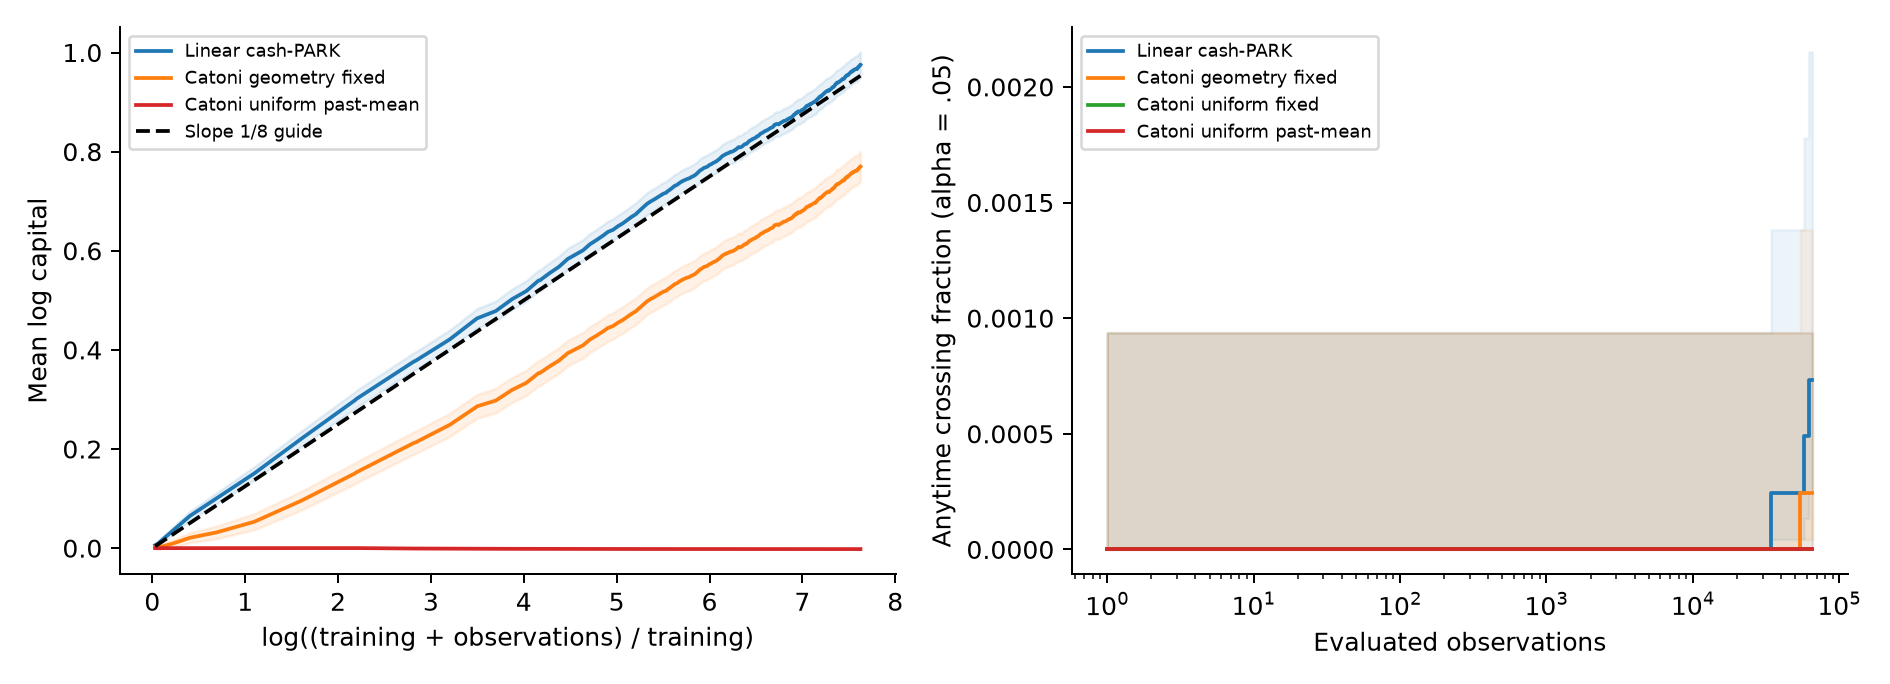
\includegraphics[width=\linewidth]{figures/vanishing_gain.png}

\caption{Scalar vanishing-gain diagnostic. Left: mean log capital with pointwise 95\% Monte Carlo intervals; the uniform fixed-bet rule is omitted from this panel because its large negative values obscure the other series. The $1/8$ line is a slope guide, not an exact finite-horizon formula. Right: all-date crossing fractions at level 5\% with pointwise Wilson intervals. Bands are not simultaneous over time.}\label{fig:vanishing}\end{figure}

Eventual crossing and a sharp confidence exponent can coexist with very low finite-horizon power. The experiment supplies no financial performance improvement or adaptation theorem for changing regimes.

